\documentclass[11pt,a4paper]{report}%especifica o tipo de documento que tenciona escrever: carta, artigo, relatório... neste caso é um relatório
% [11pt,a4paper] Define o tamanho principal das letras do documento. caso não especifique uma delas, é assumido 10pt
% a4paper -- Define o tamanho do papel.
\usepackage{float}
\usepackage[portuges]{babel}%Babel -- irá activar automaticamente as regras apropriadas de hifenização para a língua todo o
                                   %-- o texto gerado é automaticamente traduzido para Português.
                                   %  Por exemplo, “chapter” irá passar a “capítulo”, “table of contents” a “conteúdo”.
                                   % portuges -- específica para o Português.
\usepackage[utf8]{inputenc} % define o encoding usado texto fonte (input)--usual "utf8" ou "latin1

\usepackage{graphicx} %permite incluir graficos, tabelas, figuras
\usepackage{url} % para utilizar o comando \url{}
\usepackage{enumerate} %permite escolher, nas listas enumeradas, se os iems sao marcados com letras ou numeros-romanos em vez de numeracao normal

%\usepackage{apalike} % gerar biliografia no estilo 'named' (apalike)

\usepackage{color} % Para escrever em cores
\usepackage{multirow} %tabelas com multilinhas
\usepackage{array} %formatação especial de tabelas em array

\usepackage[pdftex]{hyperref} % transformar as referências internas do seu documento em hiper-ligações.

%Exemplos de fontes -- nao e vulgar mudar o tipo de fonte
%\usepackage{tgbonum} % Fonte de letra: TEX Gyre Bonum
%\usepackage{lmodern} % Fonte de letra: Latin Modern Sans Serif
%\usepackage{helvet}  % Fonte de letra: Helvetica
%\usepackage{charter} % Fonte de letra:Charter

\definecolor{saddlebrown}{rgb}{0.55, 0.27, 0.07} % para definir uma nova cor, neste caso 'saddlebrown'

\usepackage{listings}  % para utilizar blocos de texto verbatim no estilo 'listings'
%paramerização mais vulgar dos blocos LISTING - GENERAL
\lstset{
	basicstyle=\small, %o tamanho das fontes que são usadas para o código
	numbers=left, % onde colocar a numeração da linha
	numberstyle=\tiny, %o tamanho das fontes que são usadas para a numeração da linha
	numbersep=5pt, %distancia entre a numeração da linha e o codigo
	breaklines=true, %define quebra automática de linha
    frame=tB,  % caixa a volta do codigo
	mathescape=true, %habilita o modo matemático
	escapeinside={(*@}{@*)} % se escrever isto  aceita tudo o que esta dentro das marcas e nao altera
}
%
%\lstset{ %
%	language=Java,							% choose the language of the code
%	basicstyle=\ttfamily\footnotesize,		% the size of the fonts that are used for the code
%	keywordstyle=\bfseries,					% set the keyword style
%	%numbers=left,							% where to put the line-numbers
%	numberstyle=\scriptsize,				% the size of the fonts that are used for the line-numbers
%	stepnumber=2,							% the step between two line-numbers. If it's 1 each line
%											% will be numbered
%	numbersep=5pt,							% how far the line-numbers are from the code
%	backgroundcolor=\color{white},			% choose the background color. You must add \usepackage{color}
%	showspaces=false,						% show spaces adding particular underscores
%	showstringspaces=false,					% underline spaces within strings
%	showtabs=false,							% show tabs within strings adding particular underscores
%	frame=none,								% adds a frame around the code
%	%abovecaptionskip=-.8em,
%	%belowcaptionskip=.7em,
%	tabsize=2,								% sets default tabsize to 2 spaces
%	captionpos=b,							% sets the caption-position to bottom
%	breaklines=true,						% sets automatic line breaking
%	breakatwhitespace=false,				% sets if automatic breaks should only happen at whitespace
%	title=\lstname,							% show the filename of files included with \lstinputlisting;
%											% also try caption instead of title
%	escapeinside={\%*}{*)},					% if you want to add a comment within your code
%	morekeywords={*,...}					% if you want to add more keywords to the set
%}

\usepackage{xspace} % deteta se a seguir a palavra tem uma palavra ou um sinal de pontuaçao se tiver uma palavra da espaço, se for um sinal de pontuaçao nao da espaço

\parindent=0pt %espaço a deixar para fazer a  indentação da primeira linha após um parágrafo
\parskip=2pt % espaço entre o parágrafo e o texto anterior

\setlength{\oddsidemargin}{-1cm} %espaço entre o texto e a margem
\setlength{\textwidth}{18cm} %Comprimento do texto na pagina
\setlength{\headsep}{-1cm} %espaço entre o texto e o cabeçalho
\setlength{\textheight}{23cm} %altura do texto na pagina

% comando '\def' usado para definir abreviatura (macros)
% o primeiro argumento é o nome do novo comando e o segundo entre chavetas é o texto original, ou sequência de controle, para que expande
\def\darius{\textsf{Darius}\xspace}
\def\antlr{\texttt{AnTLR}\xspace}
\def\pe{\emph{Publicação Eletrónica}\xspace}
\def\titulo#1{\section{#1}}    %no corpo do documento usa-se na forma '\titulo{MEU TITULO}'
\def\super#1{{\em Supervisor: #1}\\ }
\def\area#1{{\em \'{A}rea: #1}\\[0.2cm]}
\def\resumo{\underline{Resumo}:\\ }

%\input{LPgeneralDefintions} %permite ler de um ficheiro de texto externo mais definições

\title{Projeto de System Deployment \& Benchmarking\\
       \textbf{Instalação Zulip}\\ Relatório de Desenvolvimento
       } %Titulo do documento
%\title{Um Exemplo de Artigo em \LaTeX}
\author{José André Martins Pereira\\ (a82880@alunos.uminho.pt) \and Ricardo André Gomes Petronilho\\ (a81744@alunos.uminho.pt) \and Miguel Raposo Dias\\ (pg41089@alunos.uminho.pt) \and
Ricardo Cunha Dias \\ (pg39295@alunos.uminho.pt)
       } %autores do documento
\date{\today} %data

\usepackage{hyperref}
\hypersetup{
    colorlinks=true,
    linkcolor=blue,
    filecolor=magenta,      
    urlcolor=blue,
}
 
\urlstyle{same}

\begin{document} % corpo do documento

\begin{figure}
    \centering
    
\includegraphics{images/uminho.png}
\end{figure}

\maketitle % apresentar titulo, autor e data

\tableofcontents % Insere a tabela de indice
%\listoffigures % Insere a tabela de indice figuras
%\listoftables % Insere a tabela de indice tabelas

\chapter{Introdução} \label{chap:intro} %referência cruzada
Na unidade curricular de \textbf{Systems Deployment \& Benchmarking} foi-nos proposto um trabalho prático de análise, deployment e benchmarking de uma aplicação.Ao longo deste relatório apresentam-se os processos efetuados para a concretização do projeto. \newline 

Inicialmente faz-se uma contextualização do problema e apresentação dos objetivos, descreve-se a arquitetura e componentes da aplicação, identifica-se e apresenta-se as ferramentas utilizadas na instalação e deployment da mesma. \newline 

Por fim, e não menos importante, identificam-se as ferramentas utilizadas na monitorização e benchmark, bem como se faz uma análise dos resultados obtidos.

\chapter{Contextualização do Problema}

\section{Objetivos}
Os objetivos centrais deste projeto são analisar a arquitetura de uma aplicação, para se perceber os possíveis pontos críticos, e que soluções existem, para reduzir o impacto dos mesmos. Com a resolução destes problemas, consegue-se uma maior disponibilidade da aplicação. Do mesmo modo, monitorizar e analisar o desempenho da aplicação, para diferentes configurações dos componentes, para se entender o impacto que estas tem no desempenho da aplicação.

\section{Aplicação}

\begin{figure}[h!]
\centering

\includegraphics[scale=0.30]{images/zulip.png}
\caption{Logotipo do \href{https://zulipchat.com}{Zulip}.}
\label{img:docker}
\end{figure}
\newline

Assim, a aplicação escolhida pela equipa foi o \textbf{\href{https://zulipchat.com}{Zulip}}, na medida em que segue os requisitos do trabalho prático, bem como, tem uma boa documentação.

O \textbf{Zulip} é uma aplicação de chat em tempo real, onde o principal objetivo é oferecer um boa experiência a organizações, empresas e projetos voluntários, de pequenas equipas de amigos, até dezenas de milhares de utilizadores.\\

\chapter{Arquitetura da aplicação Zulip}

A arquitetura da aplicação \textbf{zulip} contém vários \textbf{componentes}, sendo que, se consegue dividir os mesmos em diferentes subsistemas. No entanto, é perceptível pela figura \ref{img:arquitetura-zulip}, que existe uma separação entre o componente \textbf{Client} com os restantes, pois são subsistemas distintos.
\newline

\begin{figure}[H]
	\centering
	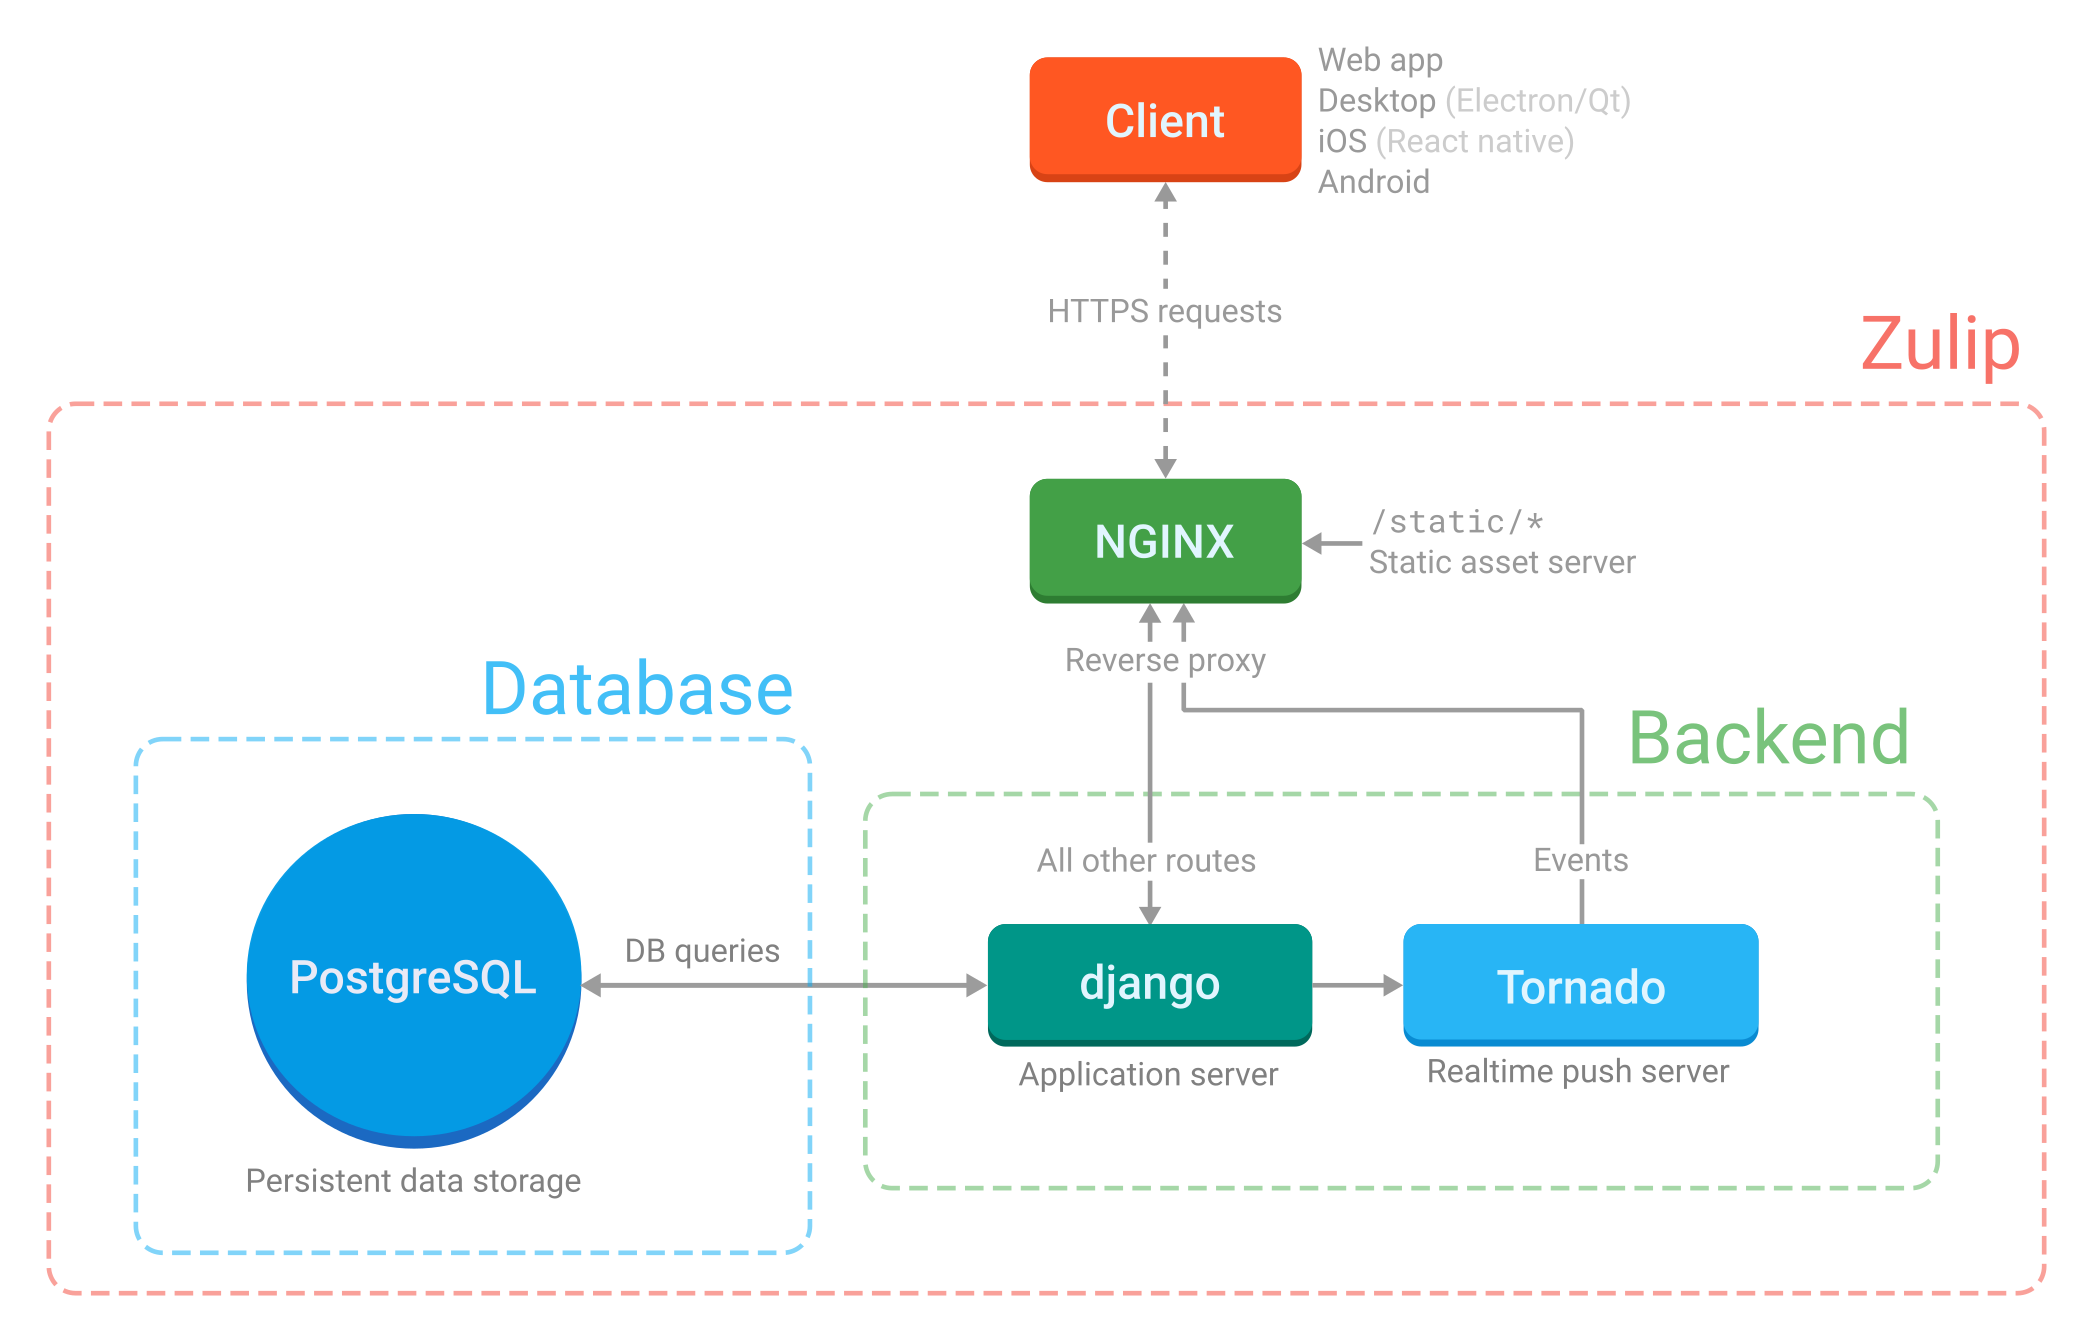
\includegraphics[scale=0.28]{images/architecture.png}
	\caption{\href{https://zulip.readthedocs.io/en/latest/overview/architecture-overview.html}{Arquitetura da aplicação Zulip.}}
	\label{img:arquitetura-zulip}
\end{figure}

O \textbf{Client} é responsável pela apresentação (\emph{view}) da aplicação, enquanto que o restante subsistema é de uma forma geral, responsável pela lógica e tratamento de dados da mesma, sendo este mais complexo e composto por subsistemas interiores (\textbf{Database} \& \textbf{Backend}).
\newline

A divisão também deve-se ao facto do componente \textbf{Client} estar na máquina do utilizador, enquanto que os restantes estarão em máquinas administradas pela empresa de desenvolvimento.
\newline

O componente \textbf{NGINX} consiste num servidor \emph{HTTP} intermediário (\emph{middleware}) entre o componente \textbf{Client} com \emph{HTTP requests} e o \textbf{Backend}. Na verdade, o \textbf{NGINX} permite uma independência entre os subsistemas, ou seja, o \textbf{Client}, pode ser definido para diferentes plataformas, nomeadamente: web, desktop, iOS e android.
\newline

Em relação à base de dados da aplicação, tem-se o componente \textbf{PostgreSQL}, um sistema de gerenciamento de dados persistente que apenas comunica com o servidor da aplicação \textbf{django}.
\newline

Em termos do sistema de \textbf{backend} da aplicação, este é composto por duas componentes, sendo elas \textbf{django} e \textbf{Tornado}, este primeiro \textbf{django} é de extrema importância tendo em conta que é a base da construção da aplicação \textbf{zulip}, e consiste num framework de web do lado do servidor de código aberto, desenvolvido em Python, fornecendo assim todo o framework necessário para ser mais tarde apresentado do lado do cliente, quanto ao \textbf{Tornado} é um servidor de web assíncrono e sem bloqueio de I/o que permite manter ativas milhares de ligações em tempo real, no caso do \textbf{zulip} é respónsavel pela entrega de mensagens e não muito mais.\\ 

Outros componentes secundários igualmente importantes no funcionamento do \textbf{zulip} são \textbf{Supervisor} que é um sistema cliente/servidor que permite monitorizar e controlar os processos em sistemas \textbf{unix}, no caso do \textbf{zulip} é utilizado para iniciar os processos do servidor, reinicializar-los em caso de falha e fazer \emph{logging}, outro é \textbf{memcached} é um sistema distribuído de cache em memória, é usado para guardar em chache modelos de dados e invalidar-los caso sejam alterados.\\

Um outro componente secundário é a base de dados em memória \textbf{Redis} que armazena chaves com durabilidade opcional, é usado para guardar dados com tempo de vida bastante baixo.\\ O \textbf{RabbitMQ} é um software de mensagens com código aberto, que é usado para tratar de filas que requerem uma entrega fiável mas não são passíveis de fazer no sistema principal, é também usado para comunicações entre \textbf{django} e \textbf{Tornado}.\\ Por último, o componente \textbf{Thumbor} é um serviço de miniaturas de fotos open-source que tem como função administrar as fotos do sistemas ora via \textbf{upload} ora via \textbf{url}.\newline

Importante realçar que a arquitetura que será elaborada no deployment da aplicação, varia consoante o número de replicas de cada componente. No entanto isto será abordado com mais detalhe nos capítulos seguintes.
\chapter{Instalação/Configuração da aplicação na Google Cloud}
De seguida apresenta-se o processo de instalação e configuração dos componentes da aplicação, onde foram utilizadas as ferramentas: \textbf{Docker}, \textbf{Kubernetes}. 

\section{Vantagens da utilização de Containers}
A utilização de containers na infraestrutura da aplicação \textbf{zulip}, permite um isolamento dos componentes, bem como um melhor aproveitamento dos recursos de cada máquina, facilitando o processo de teste, \emph{provisining} e migração dos mesmos, sendo estes importantes num processo de \textsf{deployment}.

\section{Abordagens}
Com uma análise da arquitetura da aplicação \textbf{Zulip}, percebeu-se a existência de pontos críticos (\textbf{SPOFS}).\newline Na verdade, não se deve conter num sistema componentes únicos, que em sua falta, causem a falha de todo o sistema. \newline Assim, para uma redução da probabilidade de acontecimento destes, achou-se que a solução seria a replicação dos componentes onde estes acontecem.
Operações que façam acessos à base dados, ou apenas ao servidor aplicacional, estão dependentes destes componentes, sendo crucial a fiablidade dos mesmos.
Assim, todos os componentes devem ser replicados, excepto o \textbf{NGINX}, visto a impossibilidade de replicação deste.\newline
A replicação destes componentes também contribuí para uma melhor disponibilidade, visto que, há uma distribuiçao de carga pelas várias réplicas.

\section{Docker}
A ferramenta \textbf{Docker} consiste numa plataforma para \emph{developers}, com o objetivo de construir, partihar e executar aplicações com \emph{containers}. O uso desta ferramenta facilita o processo de \textbf{deployment}.\newline As grandes vantagens do \textbf{Docker} são: 
\begin{itemize}
    \item Flexibilidade: a complexidade da aplicação não impede a possibilidade de ser colocada num container;
    \item Leves/eficientes: os recursos e kernel da máquina são partilhados por todos os containers, havendo um melhor aproveitamento dos recursos;
    \item Portabilidade: pode ser construído localmente e fazer-se o \emph{deploy} para a cloud facilmente;
    \item Escabilidade: com facilidade, consegue-se aumentar e distribuir as replicas de containers;
    \item etc ...
\end{itemize}{} 

Na figura \ref{img:docker} verifica-se uma das grandes vantagens da ferramenta \textbf{Docker} em relação à utilização de \textbf{VMs} para agregação de diferentes aplicações na mesma máquina. \newline
Tal como já foi referido, na utilização de máquinas virtuais (caso da direita da figura \ref{img:docker}), há uma repetição de sistemas operativos desnecessária para cada aplicação, e deste modo, recursos usados desnecessariamente para estes sistemas opearativos. \newline Por outro lado, no \textbf{Docker}, existe apenas um sistema operativo, partilhado por todas as aplicações, havendo assim, um melhor aproveitamento dos recursos, pois estes sao distribuídos pelos vários containers.



\begin{figure}[h!]
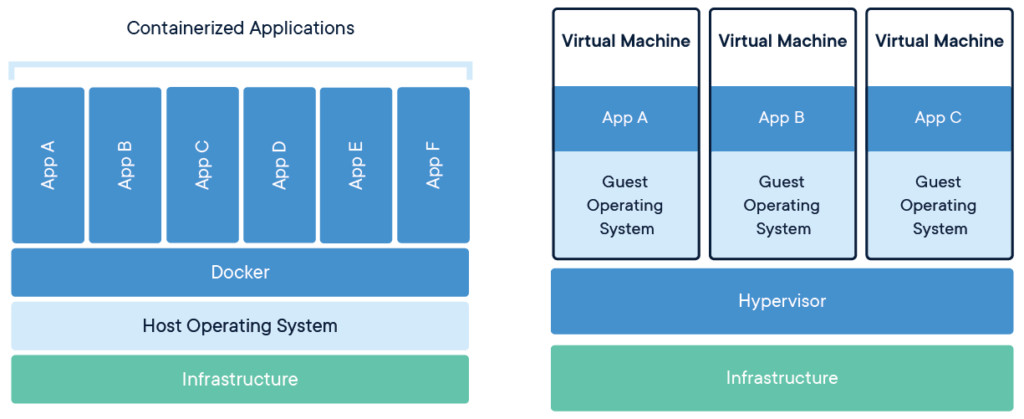
\includegraphics[scale=0.50]{images/docker.png}
\caption{Docker vs VMs.}
\centering
\label{img:docker}
\end{figure}
\newpage

\section{Kubernetes}
Trata-se de uma plataforma de código aberto, que permite gerir aplicações em containeres e automatizar a sua implementação.
\textbf{Kubernetes} introduz o conceito de \textsf{pods} que consiste em um ou mais containers.
Com a utilização do \textbf{Kubernetes}, obtem-se um \textsf{cluster}. Um cluster é um conjunto de máquinas que correm aplicações em containers, que são geridas pelo \textbf{Kubernetes}. O cluster tem pelo menos um nodo (máquina) \textsf{worker} e um \textsf{master}, sendo que o \textsf{worker} corre os \textsf{pods} que são componentes da aplicação no nosso caso \textbf{Zulip}, e o \textsf{master} gere as máquinas \textsf{worker} e os \textsf{pods} do cluster, de notar que múltiplos nós \textsf{master} permite tolerância a falhas e alta disponibilidade.
Neste caso  decidiu-se utilizar um cluster com um \textsf{master} e quatro máquinas \textsf{worker}.

\begin{figure}[h!]
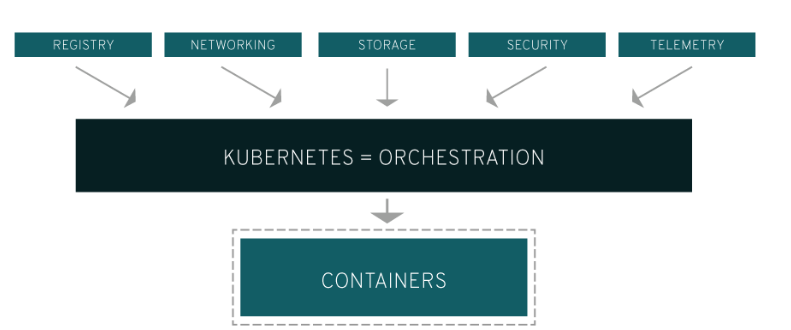
\includegraphics[scale=0.90]{images/kuber.PNG}
\caption{Arquitetura do \textbf{Kubernetes}.}
\centering
\end{figure}

\section{Automatização do Deployment}

A ferramenta \textbf{Kubernetes} facilita bastante a automatização do processo de \textbf{Deployment}, pois consegue-se definir as configurações dos componentes no ficheiro \emph{zulip-rc.yml}, em relação ao número de replicas. Com o ficheiro de configuração preparado, apenas com o comando da figura \ref{img:kub} consegue-se fazer o \textbf{Deployment} para o cluster de \textbf{Kubernetes}, onde automáticamente, os componentes são distribuídos por containers, em diferentes nodos.

\begin{figure}[h!]
\centering
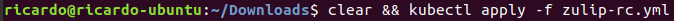
\includegraphics[scale=0.70]{images/5.png}
\caption{Comando automático para \textbf{Deployment}.}
\label{img:kub}
\end{figure}

\begin{figure}[h!]
\centering
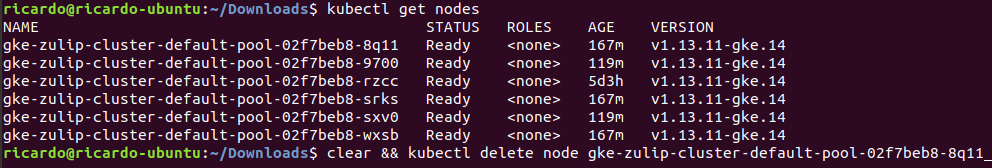
\includegraphics[scale=0.51]{images/3.png}
\caption{Comando de listar nodos, e apagar nodos.}
\end{figure}

\begin{figure}[h!]
\centering
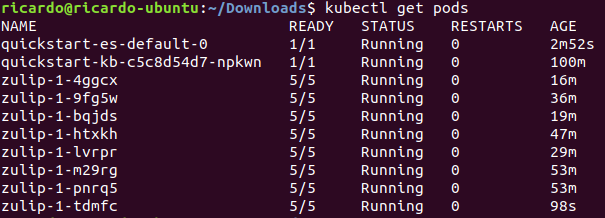
\includegraphics[scale=0.80]{images/2.png}
\caption{Listagem dos \textbf{pods}, replicas dos componentes.}
\end{figure}






\chapter{Monitorização}
As ferramentas utilizadas para Monitorização da infraestrutura foi: \textbf{MetricBeat}, como colecionador e \emph{parser} de dados, \textbf{ElasticSearch}, para analisar (\emph{RESTful search and analytics}) e por fim o \textbf{Kibana}, para visualização dos dados. \newline
Inicialmente, começou-se por criar uma máquina para monitorização, com os componentes \textbf{ElasticSearch} e \textbf{Kibana}, mas ao tentar-se instalar os \textbf{MetricBeats} nos nós do cluster, não se conseguiu. Isto deveu-se ao facto de se estar a usar o \textbf{Kubernetes}, e o mesmo estar preparado para instalar estes componentes de forma automática em containers. \newline 

Apesar da instalação do \textbf{Elasticsearch} e \textbf{Kibana} terem funcionado com \textbf{Kubernetes}, novamente a equipa teve problemas com o \textbf{MetricBeats}, pelo que devido à falta de tempo para conclusão do projeto, decidiu-se usar as métricas de monitorização fornecidas pelo \textbf{Google Cloud}.\newline 

Assim, deste modo, verifica-se que uma das necessidade de métricas, em que a monitorização foi útil, foi a deteção de falta de memória \textbf{RAM}, tal como se pode ver na figura \ref{img:monitorizacao} , quando se testou diferentes configurações dos componentes na fase de \textbf{benchmark}. 

\begin{figure}[h!]
\centering
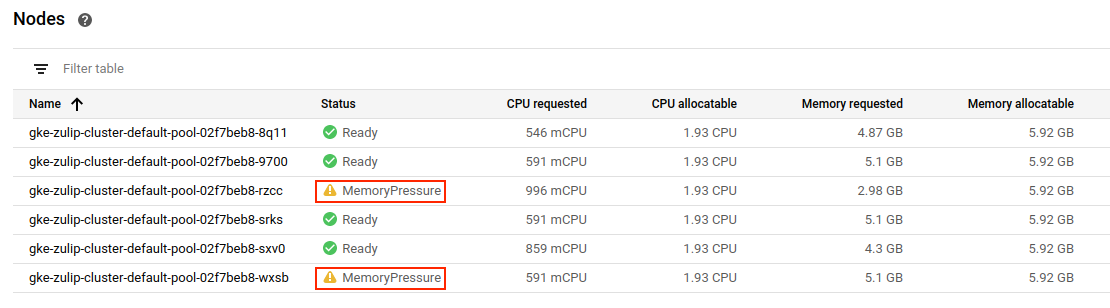
\includegraphics[scale=0.45]{images/monitorizacao.png}
\caption{Monitorização do Google Cloud.}
\label{img:monitorizacao}
\end{figure}

\chapter{Benchmarking}

Após a configuração da arquitetura e deployment do sistema foi efetuado o \textbf{benchmarking} simultâneamente à monitorização, desta forma é possível analisar com \textbf{dados concretos} se a arquitetura atual é \textbf{eficiente} para o uso \textbf{realista} da aplicação zulip por parte de vários clientes. Note-se que não é pretendido ter o sistema com os melhores recursos possíveis, isso seria dispendioso, pretende-se ter recursos suficientes para responder aos pedidos dos clientes atendendo ao binómio \textbf{custo vs rapidez}.
\newline

Foi efetuado 1 \textbf{HTTP(S) request}:

\begin{enumerate}
  \item \label{itm:fst} obtenção página inical: method \textbf{GET} https://zulip/login/
\end{enumerate}

O request foi analisado com o programa \textbf{jmeter} e efetuado com 9 configurações que variam entre o \textbf{número de clientes} e \textbf{número de pedidos de cada cliente} a cada momento. Desta forma os resultados obtidos em relação ao \textbf{número de pedidos por minuto} (throughput)que a aplicação zulip consegue atender e o respetivo tempo total encontram-se nas seguintes tabelas.

\begin{table}[H]
    \centering
    \begin{tabular}{|l||r||r|}
    \hline
        \#Clientes + \#Pedidos & Throughput & Tempo Total\\ \hline \hline
        250 C + 1 P & 65 217 & menos de 1 seg \\ \hline
        250 C + 5 P & 186 567 & menos de 1 seg \\ \hline
        250 C + 10 P & 268 817 & menos de 1 seg \\ \hline
        \hline
        500 C + 1 P & 68 965 & menos de 1 seg \\ \hline
        500 C + 5 P & 72 011 & 2 segs \\ \hline
        500 C + 10 P & 223 665 & 2 seg \\ \hline
        \hline
        1000 C + 1 P & 37 243 & 1 seg \\ \hline
        1000 C + 5 P & 73 511 & 4 segs \\ \hline
        1000 C + 10 P & 180 018 & 5 segs \\ \hline
        
    \end{tabular}
    \caption{Resultados para o HTTP(S) request \ref{itm:fst} (página incial).}
    \label{tab:testeFront}
\end{table}

A topologia final utilizada para estes teste consiste em \textbf{6 nodos} e \textbf{7 réplicas}, note-se que cada réplica utiliza 5 serviços/ containers, logo na realidade a arquitetura consiste em \textbf{6 nodos} e \textbf{35 containers}.

O benchmarking \textbf{foi essencial para otimizar a configuração dos recursos} necessária para o funcionamento fluído da aplicação. 

Inicialmente a configuração era de \textbf{3 nodos} e \textbf{1 réplica} apenas, quando foi analisado HTTP(S) request \ref{itm:fst} verificou-se o seguinte resultado.

\begin{table}[H]
    \centering
    \begin{tabular}{|l||r||r|}
    \hline
        \#Clientes + \#Pedidos & Throughput & Tempo total \\ \hline \hline
        1000 C + 1 P & 457 & 120 segs \\ \hline
    \end{tabular}
    \caption{Resultados para o HTTP(S) request \ref{itm:fst} para \textbf{3 nodos} e \textbf{1 réplica}.}
    \label{tab:testeFront}
\end{table}

Este resultado é péssimo para uma aplicação que à partida é utilizada por muitos clientes simultâneamente, uma vez que uma espera de 2 minutos é impensável, logo foi alterada a topologia, decidiu-se analisar o mesmo HTTP(S) request para várias configurações.

\begin{table}[H]
    \centering
    \begin{tabular}{|l||r||r|}
    \hline
        \#Clientes + \#Pedidos & Throughput & Tempo total \\ \hline \hline
        1000 C + 1 P & 37 428 & 1 seg \\ \hline
    \end{tabular}
    \caption{Resultados para o HTTP(S) request \ref{itm:fst} para \textbf{6 nodos} e \textbf{4 réplicas}.}
    \label{tab:testeFront}
\end{table}

\begin{table}[H]
    \centering
    \begin{tabular}{|l||r||r|}
    \hline
        \#Clientes + \#Pedidos & Throughput & Tempo total \\ \hline \hline
        1000 C + 1 P & 33 783 & 1 seg \\ \hline
    \end{tabular}
    \caption{Resultados para o HTTP(S) request \ref{itm:fst} para \textbf{6 nodos} e \textbf{7 réplicas}.}
    \label{tab:testeFront}
\end{table}

\begin{table}[H]
    \centering
    \begin{tabular}{|l||r||r|}
    \hline
        \#Clientes + \#Pedidos & Throughput & Tempo total \\ \hline \hline
        1000 C + 1 P & 71 942 & menos de 1 seg \\ \hline
    \end{tabular}
    \caption{Resultados para o HTTP(S) request \ref{itm:fst} para \textbf{6 nodos} e \textbf{8 réplicas}.}
    \label{tab:testeFront}
\end{table}

\begin{table}[H]
    \centering
    \begin{tabular}{|l||r||r|}
    \hline
        \#Clientes + \#Pedidos & Throughput & Tempo total \\ \hline \hline
        1000 C + 1 P & 39 040 & 1 seg \\ \hline
    \end{tabular}
    \caption{Resultados para o HTTP(S) request \ref{itm:fst} para \textbf{6 nodos} e \textbf{10 réplicas}.}
    \label{tab:testeFront}
\end{table}

\begin{table}[H]
    \centering
    \begin{tabular}{|l||r||r|}
    \hline
        \#Clientes + \#Pedidos & Throughput & Tempo total \\ \hline \hline
        1000 C + 1 P & 574 & 112 segs \\ \hline
    \end{tabular}
    \caption{Resultados para o HTTP(S) request \ref{itm:fst} para \textbf{8 nodos} e \textbf{8 réplicas}.}
    \label{tab:testeFront}
\end{table}

Conclui-se que a melhor configuração seria \textbf{6 nodos} e \textbf{8 réplicas}, no entanto após algum tempo com a configuração ativa notou-se que por certos períodos de tempo, existia pressão na memória RAM, tornando a aplicação mais lenta e por vezes o servidor parava, desta forma testou-se a topologia com \textbf{6 nodos} e \textbf{7 réplicas} e após bons resultados ficou a topologia final.

\chapter{Conclusão}

Em suma, conclui-se que alguns dos objetivos inicialmente propostos foram atingidos, tais como, análise da arquitetura, análise dos pontos críticos, instalação/deployment da aplicação e benchmark.\newline  

No entanto, em relação à monitorização, não se conseguiu instalar as aplicações necessárias para a mesma, mais especificamente, o \textbf{MetricBeat} em cada nodo. \newline Como alternativa, e devido à falta de tempo, a equipa baseou-se na ferramenta de monitorização da \textbf{Google Cloud}, mais propriamente \textbf{GKE - Google Kubernetes Engine}, que disponibiliza algumas métricas, apesar de que em menos quantidade, foram bastante úteis, tal como já foi dito, no momento de teste de diferentes configuraçõe dos componentes da aplicação, para deteção de falta de \textbf{RAM}.\\

A utilização de kubernetes, facilitou o processo de automatização do \textbf{Deployment} da aplicação, bem como das alterações da configuração dos componentes, tornando possíveis instalações para produção mais facilitadas.

A análise de benchmark da aplicação apesar de se conseguir boas conclusões dos resultados, poderia ter sido feita com mais funcionalidades, mas devido à falta de tempo, não foi possível.

Após os resultados obtidos nas várias configurações dos componentes, dos benchmarks, verificou-se que a melhor configuração, a nível performance, consiste seis nodos e sete replicas de cada componente.

Por fim, e não menos importante a análise dos pontos críticos da aplicação passou por uma análise da arquitetura da mesma e identifcar possíveis problemas. Os principais problemas encontrados foram a não tolerância a faltas de determinados componentes, que compromentem todo o sistema.

\end{document}
